%%%%%%%%%%%%%%%%%%%%%%%%%%%%%%%%%%%%%%%%%%%%%%%%%%%%%%%%%%%%%%%%%%%%%%%%%%%%%%%%
%2345678901234567890123456789012345678901234567890123456789012345678901234567890
%        1         2         3         4         5         6         7         8

\documentclass[letterpaper, 10 pt, conference]{ieeeconf}  % Comment this line out if you need a4paper

%\documentclass[a4paper, 10pt, conference]{ieeeconf}      % Use this line for a4 paper

\IEEEoverridecommandlockouts                              % This command is only needed if 
                                                          % you want to use the \thanks command

\overrideIEEEmargins                                      % Needed to meet printer requirements.

% See the \addtolength command later in the file to balance the column lengths
% on the last page of the document

% The following packages can be found on http:\\www.ctan.org
\usepackage{graphicx} % for pdf, bitmapped graphics files
\usepackage{subcaption}
% \usepackage{epsfig} % for postscript graphics files
%\usepackage{mathptmx} % assumes new font selection scheme installed
%\usepackage{times} % assumes new font selection scheme installed
%\usepackage{amsmath} % assumes amsmath package installed
%\usepackage{amssymb}  % assumes amsmath package installed

\title{\LARGE \bf
A Quadratic Program Controller for the ATRIAS Point-Footed Biped*
}


\author{Laura Hallock$^{1}$ and Veronica Lane$^{2}$% <-this % stops a space
\thanks{*This work was completed as a final project for MIT 6.832 Underactuated Robotics, Fall 2014.}% <-this % stops a space
\thanks{$^{1}$Laura Hallock is an undergraduate student of Electrical Engineering and Computer Science,
        Massachusetts Institute of Technology, Cambridge, MA, USA
        {\tt\small lhallock@mit.edu}}%
\thanks{$^{2}$Veronica Lane is an undergraduate student of Electrical Engineering and Computer Science,
        Massachusetts Institute of Technology, Cambridge, MA, USA
        {\tt\small vmlane@mit.edu}}%
}


\begin{document}



\maketitle
\thispagestyle{empty}
\pagestyle{empty}


%%%%%%%%%%%%%%%%%%%%%%%%%%%%%%%%%%%%%%%%%%%%%%%%%%%%%%%%%%%%%%%%%%%%%%%%%%%%%%%%
\begin{abstract}

We implement a whole-body dynamic walking controller which uses a convex quadratic program for the ATRIAS point-footed biped robot in simulation. The controller attempts to minimize an objective function while maintaining input, contact, dynamic, and no-slip constraints. We attempt to demonstrate that the Zero Moment Point (ZMP) stability criterion can apply to a point footed biped.

\end{abstract}


%%%%%%%%%%%%%%%%%%%%%%%%%%%%%%%%%%%%%%%%%%%%%%%%%%%%%%%%%%%%%%%%%%%%%%%%%%%%%%%%
\section{INTRODUCTION \& PROBLEM FORMULATION}

An agile biped robot capable of walking and running over rough terrain has a wide variety of applications, including search and rescue operations and exploration. A biped robot is underactuated and the robot cannot execute an arbitrary trajectory in all degrees of freedom. Because of this, conventional controls do not work and the dynamics of walking robots pose a difficult challenge.

\section{MOTIVATION}

A Quadratic Program (QP) Controller uses the Zero Moment Point (ZMP) stability criterion.  The ZMP is a point on the ground where the reaction forces from the contact points of the feet on the ground produce no horizontal moment. In other words, the ground and inertial forces sum horizontally to zero and the moment produced by these forces is perpendicular to the ground plane. Furthermore, ZMP assumes that at least one foot is on the ground at all times. There is debate in the robotics community about whether or not the ZMP stability criterion will work for a point footed-biped, since there is no support polygon. We aim to prove that the ZMP stability criterion is an valid for a point-footed biped by developing a QP controller for ATRIAS, which will enable it to execute walking trajectories over flat terrain.

For our project, we chose to test the efficacy of a QP controller on the ATRIAS biped, a point-footed robot that is highly articulated enough to merit such a sophisticated control system. We chose ATRIAS due both to its similarities to Atlas --- as they are both bipeds with a sophisticated, non-flat-footed gait --- and because we had access to the existing URDF files to describe the robot.

\section{PREVIOUS WORK}

   \begin{figure}[thpb]
      \centering
      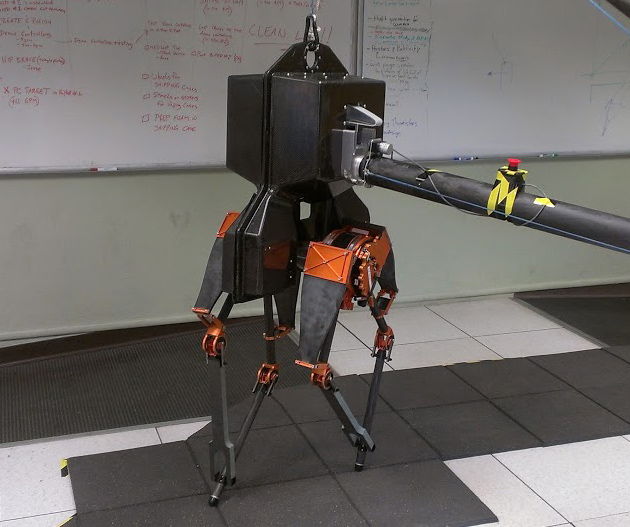
\includegraphics[scale=0.3]{figures/atrias.jpg}
      \caption{The ATRIAS biped.}
      \label{atrias}
   \end{figure}

\subsection{The ATRIAS Biped}

The ATRIAS biped --- short for “Assume The Robot Is A Sphere,” a design paradigm used by creator Jonathan Hurst --- represents the third iteration, following several monopods, of the ATRIAS series of robots developed at Oregon State University. The series was designed for walking and running over uneven, unpredictable terrain while maintaining a reasonably economy of energy. \cite{site1} Although most of the published successes in control systems restrict ATRIAS to operating on a boom, the ATRIAS biped is designed to ultimately walk and run untethered. Under University of Michigan Professor Jessy Grizzle, researchers are currently working toward this goal on MARLO, an iteration of ATRIAS with prosthetic feet. MARLO has successfully taken steps, both in the lab and outdoors, while tethered to a gantry. \cite{site2}

The ATRIAS robot has 6 actuators and 13 degrees of freedom. It is designed as a Spring Mass Loaded Inverted Pendulum (SLIP).
For our project, we made use of several URDF files of ATRIAS created by Professor Grizzle when he visited MIT. As discussed below, we made extensive modifications to these files, including the removal of several linkages and the addition of actuators.

\subsection{Previous Controllers}

Researchers at Carnegie Mellon developed a controller for ATRIAS using a spring-mass model (SMM). SMM was chosen to describe ATRIAS's locomotion dynamics because it is a good approximation for the center of mass dynamics of human running. \cite{hereid14}

  \begin{figure*}[tbp]
  \centering
  \begin{subfigure}[b]{0.7\textwidth}
    \centering
    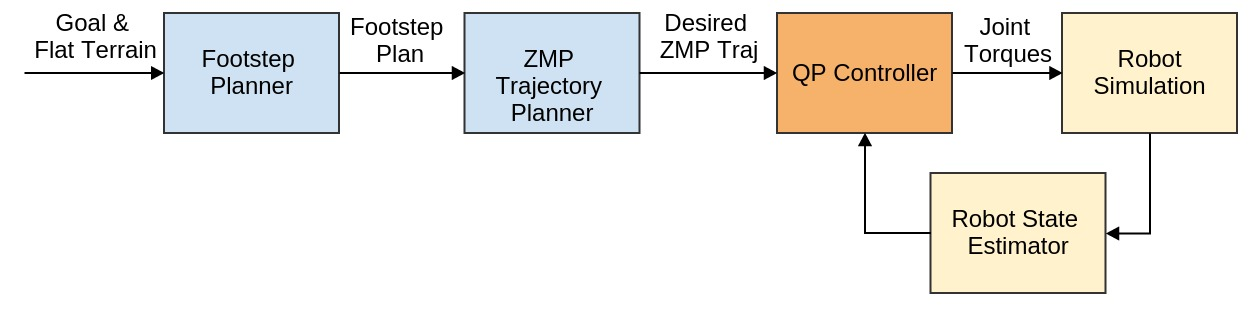
\includegraphics[width=\textwidth] {figures/6_832blockdiagramsmall.jpg}
    \label{fig:pipeline1}
  \end{subfigure}\hfill
  \caption{The algorithmic pipeline.}
  \label{fig:pipeline}
\end{figure*}

\subsection{Drake's Atlas Controller}

The MIT Robot Locomotion Group (RLG) has developed a walking trajectory planner for Atlas, a humanoid robot designed by Boston Dynamics. The planner uses ZMP as ​the stability criterion. The ZMP trajectory planner was enabled Atlas to walk, but the stability criterion assume that Atlas's center of mass remained at a constant heigh or slope. \cite{dai14} MIT's RLG developed a Quadratic Program (QP) controller for Atlas, which computes the optimal torques for each joint at each time step given the COM trajectory produced by the whole body motion planner. \cite{kuindersma13}

The QP controller is a whole-body controller that uses a convex quadratic program. It solves an optimal control problem while maintaining input, contact, no-slip, and dynamic constraints. As previously stated, maintaining the ZMP ensures dynamic stability. Given the ZMP trajectory, the time-varying LQR yields the optimal cost-to-go for a simplified model. This function is then passed to the quadratic program which solves for all torque inputs for the robot dynamics.

In creating a control system for ATRIAS, we drew heavily on the Atlas controller and walking planner already implemented in the Drake library \cite{c1}. Our specific modifications to the code for the ATRIAS model are described below.

\section{ALGORITHMIC APPROACH}

\subsection{Pipeline}

We employ the same control pipeline as Atlas to generate and execute a walking trajectory. We first generate a robot model, goal location and (flat) terrain map. These then become the inputs to the footstep planner, which outputs a set of footstep positions ending at the goal location. This plan is then analyzed by the ZMP trajectory planner, which uses inverse kinematics to calculate the trajectory of the robot’s zero-moment point. This trajectory is then passed into the QP controller, which calculates the required torques at each of ATRIAS’s actuators at each time step. This controller is then tested on the robot in simulation to determine whether it allows the robot to successfully execute the planned trajectory. \cite{dai14}\cite{deits14}

\subsection{LQR}
\begin{multiline}
\dot x = \mathbf{Ax} + \mathbf{Bu} \\
 = \left[ \begin{array}{cc}
0 & \mathbf{I}  \\
0 & 0 \end{array} \right]\] 
\left[ \begin{array}{cc}
0  \\
\mathbf{I} \end{array} \right]\] \mathbf{u}
\end{multiline}

\begin{multiline}
\mathbf{y} = \mathbf{Cx} - b(\mathbf{x},\mathbf{\dotx})\mathbf{u} \\
= \left[ \begin{array}{cc} \mathbf{I} & 0 \end{array} \right]\] \mathbf{x} - 
\frac{z_{com}}{\ddot z_{com} + g} \mathbf{Iu}
\end{multiline}


\subsection{The QP Controller}

In calculating the joint torques, we use the QP formulation used to control Atlas in Drake and documented in \cite{c1}. At each time step, we solve the quadratic program by minimizing objective function

$$
V(\bar{\mathbf{x}},\bar{\mathbf{u}},t) + w_{\ddot{\mathbf{q}}} \Vert \ddot{\mathbf{q}}_{des} - \ddot{\mathbf{q}} \Vert ^ 2 + \epsilon \sum\nolimits_{ij} \beta_{ij} ^ 2 + \Vert \eta \Vert ^ 2  \eqno{(1)}
$$

over $\ddot{q}$, $\beta$, $\lambda$, and $\eta$ subject to

$$
\mathbf{H}_{f} \ddot{\mathbf{q}} + \mathbf{C}_{f} = \Phi_{f} ^ T \lambda \eqno{(2)}
$$
$$
\mathbf{J} \ddot{\mathbf{q}} + \dot{\mathbf{J}} \dot{\mathbf{q}} = - \alpha \mathbf{J} \dot{\mathbf{q}} + \eta \eqno{(3)}
$$
$$
\mathbf{B}_{a} ^ {-1} (\mathbf{H}_{a} \ddot{\mathbf{q}} + \mathbf{C}_{a} - \Phi_{a} ^ T \lambda) \in [\tau_{min}, \tau_{max}] \eqno{(4)}
$$
$$
\forall_{j = \{1 . . . N_{c}\}} \lambda_{j} = \sum\limits_{i=1}^{N_d} \beta_{ij} \mathbf{v}_{ij} \eqno{(5)}
$$
$$
\forall_{i,j} \beta_{ij} \geq 0 \eqno{(6)}
$$
$$
\eta \in [\tau_{min}, \tau_{max}] \eqno{(7)}
$$

These constraints ensure that the dynamics and input limits (2 and 4), no-slip contact constraints (3), and contact force constraints (5 and 6) are respected. A more complete discussion of this formulation and the symbols used can be found in \cite{kuindersma13}.

The first term of the objective function $V(\bar{\mathbf{x}},\bar{\mathbf{u}},t)$ is a control Lyapunov 

\subsection{Testing Efficacy on Point-Footed Robot}

   \begin{figure}[thpb]
      \centering
      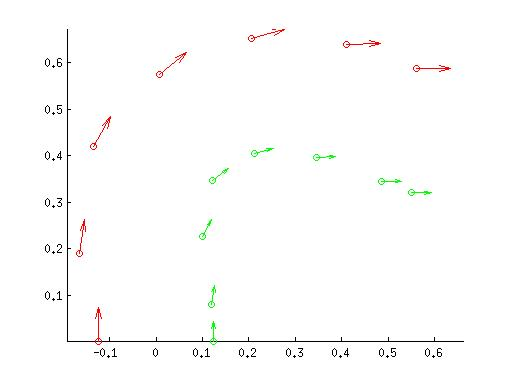
\includegraphics[scale=0.5]{figures/footstep_plan.jpg}
      \caption{An example footstep plan generated by the footstep planning block. The block takes in the robot parameters, a goal location, and a terrain map, and generates the $x$-$y$-positions of each footstep.}
      \label{footstep}
   \end{figure}

In order to work within the existing Drake infrastructure --- which requires 3-DOF feet in order to successfully plan footsteps --- we began by giving ATRIAS large, square feet. This allowed us to get the pipeline up and running without having to completely rewrite the footstep planning algorithm. Since our ultimate goal is a point-footed robot, we will then systematically shrink these feet until the QP controller ceases to work. Pending this strategy’s success, we will in future iterations of the project attempt to modify the planner such that these “dummy” feet become unnecessary.

   \begin{figure}[thpb]
      \begin{subfigure}[b]{\linewidth}
        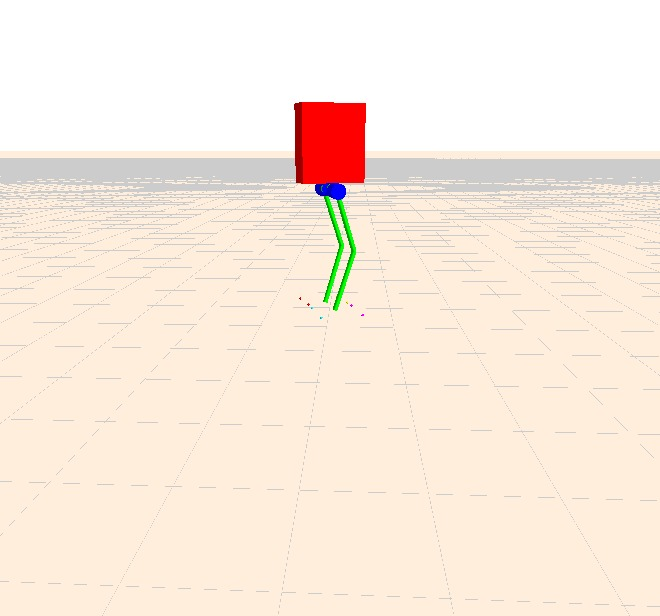
\includegraphics[width=\linewidth]{figures/runPassiveInitial.jpg}
        \caption{t = 0}
        \label{runPassiveInit}
      \end{subfigure}
      \begin{subfigure}[b]{\linewidth}
        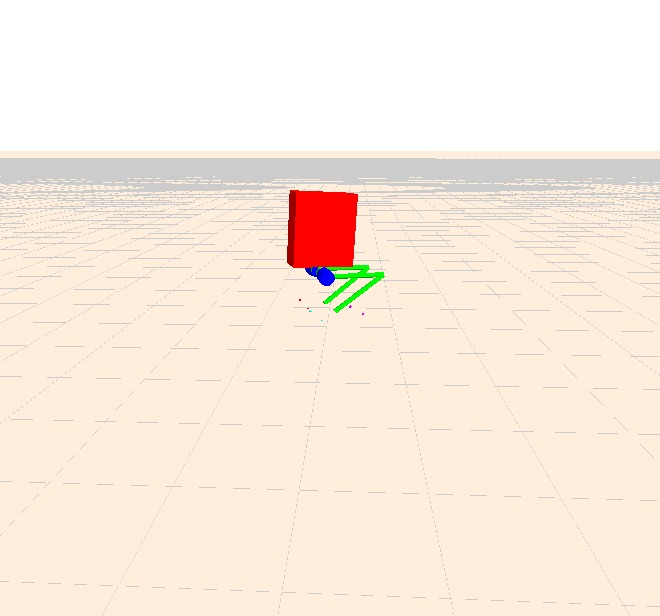
\includegraphics[width=\linewidth]{figures/runPassiveFinal.jpg}
        \caption{t = 2}
        \label{runPassiveFinal}
      \end{subfigure}
      \caption{Initial and final positions of robot in {\tt runPassive}.}
      \label{footstep}
   \end{figure}

\subsection{Subgoals and Planned Technical Approach}

To test the efficacy of our control approach at each stage in the process, we first planned to modify the ATRIAS URDF file to successfully run in simulation and ensure that all joint limits were reasonable. We then planned to use $runPassive$ to confirm that the robot ragdolls as expected when dropped. Once this was achieved, we planned to first work to use our QP controller to balance the footed ATRIAS, then confirm that we can generate a footstep plan and ZMP trajectory, and test our controller on the resulting trajectory. We then planned explore how small we can make ATRIAS's feet, as stated above.

\subsection{Modifications to Planned Technical Approach}

\begin{figure*}[tbp]
  \centering
  \begin{subfigure}[b]{0.3\textwidth}
    \centering
    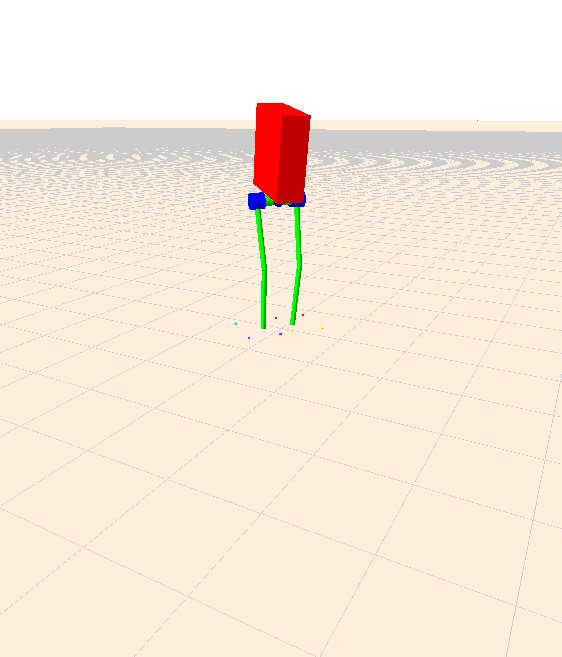
\includegraphics[width=\textwidth] {figures/balanceNoYaw1.jpg}
    \caption{t = 0}
    \label{fig:balanceNoYaw1}
  \end{subfigure}\hfill
  \begin{subfigure}[b]{0.3\textwidth}
    \centering
    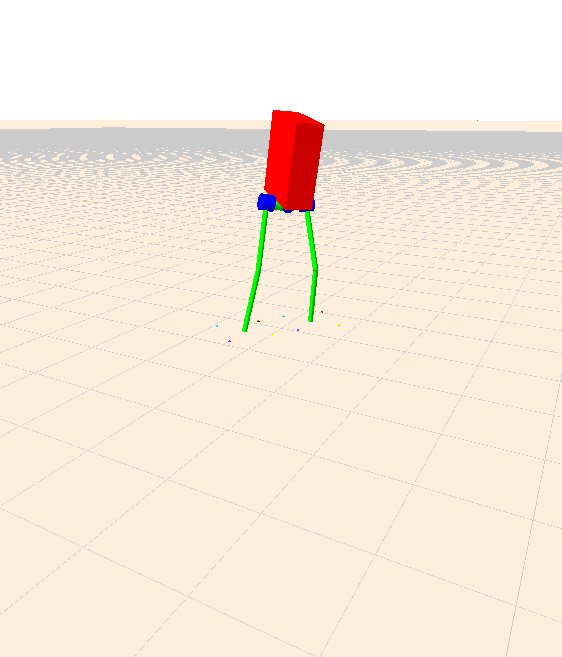
\includegraphics[width=\textwidth] {figures/balanceNoYaw2.jpg} 
    \caption{t = 1.4[s]}
    \label{fig:balanceNoYaw2}
  \end{subfigure}\hfill
  \begin{subfigure}[b]{0.3\textwidth}
    \centering
    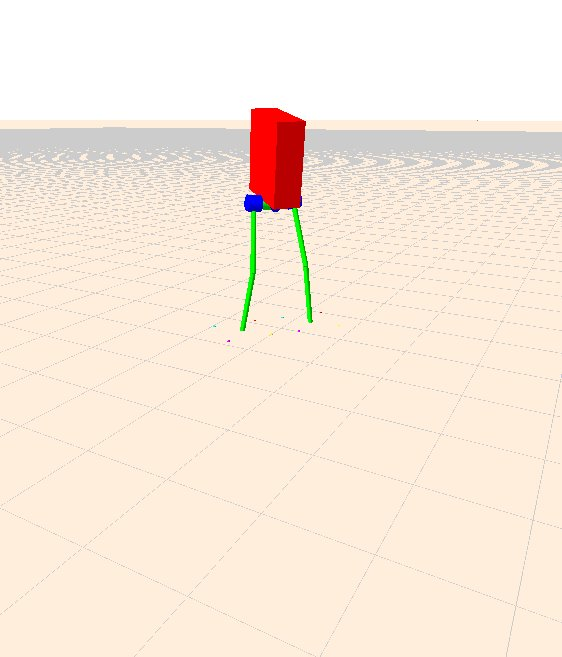
\includegraphics[width=\textwidth] {figures/balanceNoYaw3.jpg} 
    \caption{t = 2[s], error = 0.0504}
    \label{fig:balanceNoYaw3}
  \end{subfigure}
  \caption{Results for the balancing controller when ATRIAS's ankle does not have a yaw degree of freedom (DOF). The controller balance ATRIAS relatively without this DOF. }
  \label{fig:balancing}
\end{figure*}

\begin{figure*}[tbp]
  \centering
  \begin{subfigure}[b]{0.3\textwidth}
    \centering
        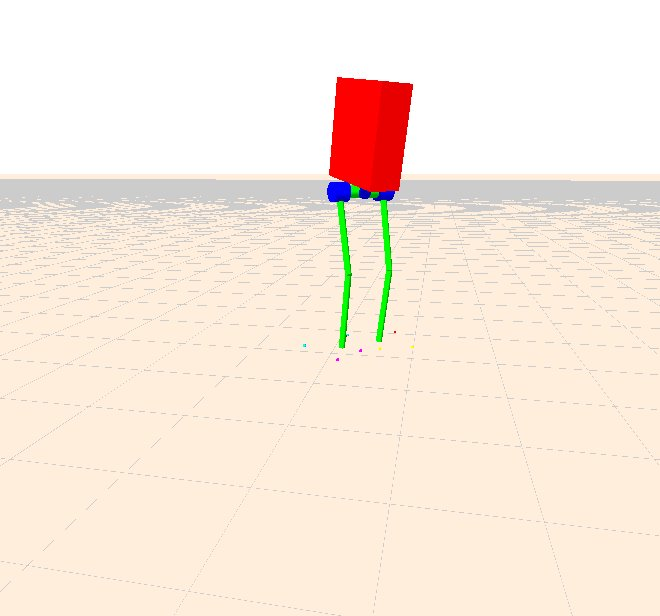
\includegraphics[width=\textwidth] {figures/balanceYaw1.jpg}
        \caption{t = 0}
    \label{fig:balanceYaw1}
    \end{subfigure}\hfill
    \begin{subfigure}[b]{0.3\textwidth}
    \centering
        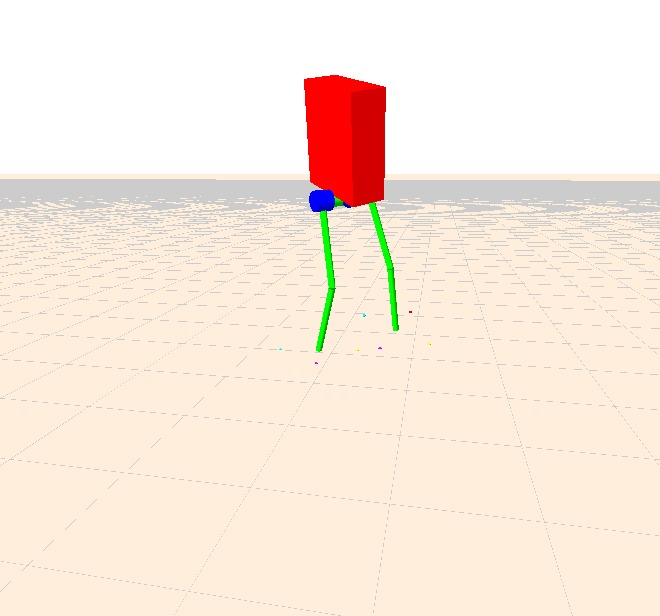
\includegraphics[width=\textwidth] {figures/balanceYaw2.jpg}
        \caption{t = 1.2[s]}
        \label{fig:balanceYaw2}
    \end{subfigure} \hfill
    \begin{subfigure}[b]{0.3\textwidth}
      \centering
        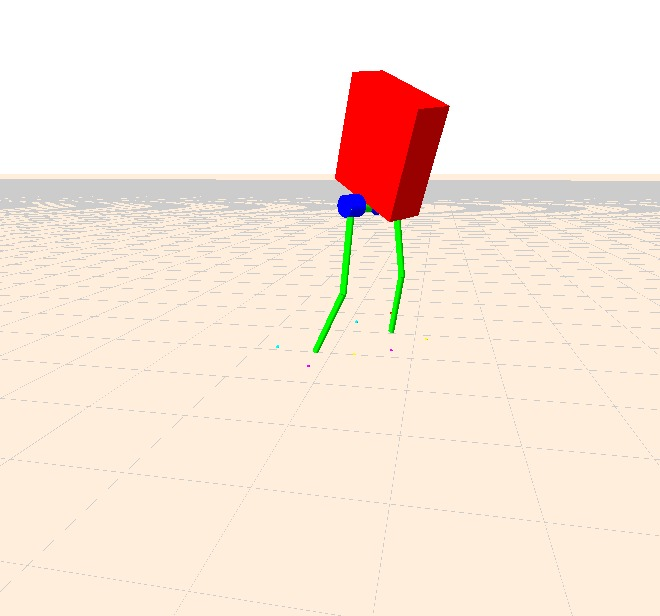
\includegraphics[width=\textwidth] {figures/balanceYaw3.jpg}
        \caption{t = 2[s], error = 0.4850}
        \label{fig:balanceYaw3}
    \end{subfigure}
  \caption{Results for the balancing controller when ATRIAS's ankle has a yaw degree of freedom. At 2 seconds, the robot begins to fall over.}
  \label{fig:balancing}
\end{figure*}


We first attempted to ensure that the URDF for ATRIAS was working by starting ATRIAS from an initial position and simulating it with no torque inputs. If successful, ATRIAS bends its knees and falls to the ground. Unfortunately, even after making significant modifications to the 4Bar model of ATRIAS, the model was unable to run passively. We then decided to switch to a simpler model with the 4Bars removed. We again had to make significant modifications to the URDF, including removing coordinate frame that was included in the URDF, adding actuators at the knees, and removing unnecessary links. Initially, we did not attempt to run a balancing controller on ATRIAS, because the initial model was point footed, and therefore the balancing controller would not work. We instead worked on make Atrias walk, we initially attempted to generate the footstep planner using the lower leg as the foot link, but this caused problems with the footstep planner. To allow both the footstep planner and controller to work, we added spheres to each of the lower-leg links to represent feet. In the URDF we added two sphere links for each leg, one for both the pitch and roll degrees of freedom. We also added small (less than 3 cm area) triangular collision groups to each foot, because the footstep planner required a support polygon in order work properly. Even after making these modifications, the footstep planner was unable to generate a footstep plan because unlike Atlas, ATRIAS’s hip doesn’t have freedom to rotate in the yaw direction. We fixed this issue by adding another spherical link and joint ot the foot to allow yaw rotation, which allowed the footstep planner to successfully generate a plan. 
Once the footstep planner was working, we adjusted the gains and parameters of the QP Controller in order to make ATRIAS walk, however, ATRIAS would immediately begin to fall over. In order to isolate the source of the error, we removed the body motion controllers for the feet and torso, and attempted to make ATRIAS walk by adjusting the IKPD gains.

First, we attempted to make ATRIAS  fall over rigidly by setting the output of the QP Controller and the input to the Ricatti equation to zero and adjusting the IKPD controller gains. No matter how the gains were adjusted ATRIAS would bend its knees each time it fell. Even after making these adjustments, ATRIAS would still fall over immediately.

We then modified the URDF to add actuators to each of the foot joints, to allow the QP controller to control the roll, pitch, and yaw of the foot. This allowed ATRIAS to balance for a longer period of time, but it still fell over before taking a single step. 

Since we could not get the robot to balance with very small triangular support polygons, we modified the contact groups in the URDF so that ATRIAS had large rectangular feet. Now that ATRIAS had feet, we decided to work on making ATRIAS balance, before trying to make it walk. The balancing test drops ATRIAS from a certain height above the ground, and attempts to make ATRIAS balance with its COM at a given location. During this test, we discovered that the URDF had no actuator at the hip, which was causing the balancing controller to fail. After adding the actuator at the hip, the robot still fell over while balancing, but was able to balance without falling over, but the error in COM location was about 15 cm, while less than 2 cm was desired. 

Given that the balancing controller worked for other bipeds, including Atlas and Hubo, we concluded that the failure of the balancing controller was due to problems with the model of the robot. We made further modifications to the URDF by removing actuators that did not move anything when viewed in the inspector and fixing the corresponding joints. This yielded slight (2-3cm) improvements in the error. We then removed the yaw degree of freedom in the foot, which resulted in significant performance improvement. The error was approximately 5 cm, as opposed to 15 cm with this degree of freedom.

\section{PROJECT STATUS}

Due to the time-intensive modifications we had to make to the ATRIAS URDF file, we have not yet been able to create a working QP controller that allows ATRIAS to walk. Currently, we have successfully generated footstep plans and are close to a working balancing controller, but we are currently debugging an issue that prevents both of these processes from successfully operating on the same URDF file. Namely, we can only achieve a reasonable result while balancing when we fix the yaw angle of each of ATRIAS’s feet. At the same time, the footstep planner explicitly plans for each foot’s position in roll, pitch, and yaw, and thus requires ATRIAS to have each of these degrees of freedom: otherwise, ATRIAS must bend its knees and apply strange torques to its hip actuators in order to keep the foot pointed forward, causing ATRIAS to infeasibly lower its center of mass and ultimately fall over.

We are currently evaluating our balancing controller with respect to the threshold used by ATLAS: i.e., we consider ATRIAS “balanced” if it remains within 2 cm of the goal fixed point after 2 s of simulation. While we have not yet been able to remain within this threshold, we have achieved an error of approximately 5 cm. At this point, when ATRIAS is dropped, the torso first leans off to one side, then appears to stabilize very precisely. We hypothesize that by further adjusting the gains to mitigate this oscillation, we can achieve better balancing precision. We are also investigating the possibility that there are still more significant problems with the URDF file that are preventing us from accurately balancing with a fixed foot yaw or from balancing at all with yaw as a DOF.

\section{LESSONS LEARNED}

Lessons learned.

\section{FUTURE WORK}
Further work will attempt to successfully implement the QP Controller for the ATRIAS biped. In order for ATRIAS walk with feet, it first must be able to balance. As previously stated, allowing the feet to rotate in the yaw direction causes the balancing controller to fail. However, removing this degree of freedom causes the footstep planner to fail. We will modify the simulated ATRIAS model to allow both the balancing controller and the footstep planner to succeed, while still accurately approximating the dynamics of ATRIAS. Once both the balancing controller and footstep planner work, we will adjust the gains and paramaters of the QP controller to make ATRIAS walk over flat terrain. 

After ATRIAS successfully walks with feet, we will incrementally decrease the size of the feet until the controller fails. For each iteration, we will adjust gains and controller parameters to make ATRIAS walk over flat terrain. When the size of the support polygon is negligible, the ATRIAS model will approximate a point-footed robot.

\section{CONCLUSIONS}

Ultimately, we were unable to progress as far toward our goal of creating a QP controller for a point-footed biped as we would have liked. By exploring the the system's failure modes, however, we learned a great deal about the intricacies of each stage in the pipeline, from URDF modeling, to footstep planning, to the QP controller itself. We gained significant intuition for what might cause a controller to fail, and we look forward to continuing this project over IAP.

\addtolength{\textheight}{-12cm}   % This command serves to balance the column lengths
                                  % on the last page of the document manually. It shortens
                                  % the textheight of the last page by a suitable amount.
                                  % This command does not take effect until the next page
                                  % so it should come on the page before the last. Make
                                  % sure that you do not shorten the textheight too much.

%%%%%%%%%%%%%%%%%%%%%%%%%%%%%%%%%%%%%%%%%%%%%%%%%%%%%%%%%%%%%%%%%%%%%%%%%%%%%%%%



%%%%%%%%%%%%%%%%%%%%%%%%%%%%%%%%%%%%%%%%%%%%%%%%%%%%%%%%%%%%%%%%%%%%%%%%%%%%%%%%



%%%%%%%%%%%%%%%%%%%%%%%%%%%%%%%%%%%%%%%%%%%%%%%%%%%%%%%%%%%%%%%%%%%%%%%%%%%%%%%%

\section*{ACKNOWLEDGMENT}

We would like to thank visiting Professor Jessy Grizzle for the ATRIAS URDF files we used in our project, as well as Professor Russ Tedrake and the entire Drake development team. Additionally, we would like to thank Dr. Scott Kuindersma, Andres Valenzuela, and Robin Deits of the MIT Robot Locomotion Group for all their help problem solving and debugging.



%%%%%%%%%%%%%%%%%%%%%%%%%%%%%%%%%%%%%%%%%%%%%%%%%%%%%%%%%%%%%%%%%%%%%%%%%%%%%%%%

\begin{thebibliography}{99}

\bibitem{site1} ATRIAS 2.1 Biped. (2012) [Online]. Available: http://mime.oregonstate.edu/research/drl/robots/atrias\_2\_1/. 

\bibitem{site2} Moore, Nicole. Two-legged robot walks outside at U-M. (2013, Dec. 3) [Online]. Available: http://www.engin.umich.edu/college/about/news/stories/2013/december/two-legged-robot-walks-outside-at-u-michigan. 

\bibitem{c1} Russ Tedrake, ÒDrake: A planning, control, and analysis toolbox for nonlinear dynamical systems,Ó  2014, http://drake.mit.edu.

\bibitem{kuindersma13} S. Kuindersma, F. Permenter, and R. Tedrake, ÒAn efficiently solvable quadratic program for stabilizing dynamic locomotion,Ó in Robotics and Automation, 2013. ICRA ’13. IEEE International Conference on, 2013.

\bibitem{dai14} Hongkai Dai, Andrés Valenzuela, and Russ Tedrake. Whole-body motion planning with centroidal dynamics and full kinematics. IEEE-RAS International Conference on Humanoid Robots, 2014. 

\bibitem{hereid14} A Hereid, S Kolathaya, MS Jones, J Van Why, JW Hurst, AD Ames. Dynamic Multi-Domain Bipedal Walking with ATRIAS through SLIP based Human-Inspired Control. Proceedings of the 17th international conference on Hybrid systems: computation and control. 2014.

\bibitem{deits14} Robin L H Deits and Russ Tedrake. Computing large convex regions of obstacle-free space through semidefinite programming. In Proceedings of the Eleventh International Workshop on the Algorithmic Foundations of Robotics (WAFR 2014), Istanbul, 2014.

\end{thebibliography}

% {\small
% \bibliographystyle{ieee}
% \bibliography{egbib}
% }

\end{document}
